\subsection{UC8: Visualizzazione della lista dei prodotti}
\label{sec:UC8}
\begin{figure}[!ht]
    \caption{Diagramma di UC8: Visualizzazione della lista dei prodotti}
    \vspace{10px}
    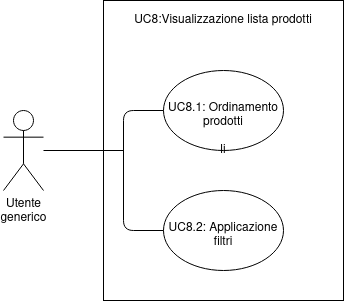
\includegraphics[scale=0.5]{../../../Images/AnalisiRequisiti/UC08.png}
    \centering
\end{figure}
\begin{itemize}
    \item \textbf{Descrizione:} l'utente visualizza la pagina della lista dei prodotti;
    \item \textbf{Attore Primario:} utente generico;
    \item \textbf{Precondizione:} l'utente si trova in una qualsiasi pagina della piattaforma;
    \item \textbf{Postcondizione:} l'utente visualizza la pagina con la lista dei prodotti;
    \item \textbf{Scenario Principale:}
          \begin{itemize}
              \item l'utente è in una pagina della piattaforma;
              \item cerca un prodotto utilizzando la barra di ricerca o scegliendo una categoria;
              \item l'utente visualizza la lista dei prodotti;
          \end{itemize}
\end{itemize}
\subsubsection{UC8.1: Ordinamento prodotti}
\label{sec:UC8.1}
\begin{itemize}
    \item \textbf{Descrizione:} l'utente seleziona la modalità in cui visualizzare i file;
    \item \textbf{Attore Primario:} utente generico;
    \item \textbf{Precondizione:} l'utente si trova all'interno della pagina con la lista dei prodotti (\hyperref[sec:UC8]{\underline{UC8}});
    \item \textbf{Input:} selezione del parametro scelto;
    \item \textbf{Postcondizione:} la lista dei prodotti si aggiorna secondo l'ordinamento scelto;
    \item \textbf{Scenario Principale:}
          \begin{itemize}
              \item l'utente si trova all'interno della pagina con la lista dei prodotti;
              \item l'utente seleziona i parametri per ordinare i prodotti;
              \item la pagina con la lista dei prodotti si aggiorna con i prodotti ordinati.
          \end{itemize}
\end{itemize}
\subsubsection{UC8.2: Applicazione filtri}
\label{sec:UC8.2}
\begin{itemize}
    \item \textbf{Descrizione:} l'utente filtra i prodotti in base alle loro caratteristiche;
    \item \textbf{Attore Primarilo:} utente generico
    \item \textbf{Precondizione:} l'utente si trova all'interno della pagina con la lista dei prodotti (\hyperref[sec:UC8]{\underline{UC8}});
    \item \textbf{Input:} selezione del filtro desiderato;
    \item \textbf{Postcondizione:} la pagina si aggiorna secondo i filtri selezionati;
    \item \textbf{Scenario Principale:}
          \begin{itemize}
              \item l'utente si trova all'interno della pagina con la lista dei prodotti;
              \item l'utente seleziona i filtri da applicare;
              \item la pagina con la lista dei prodotti si aggiorna con i prodotti filtrati.
          \end{itemize}
\end{itemize}